\chapter{Grundlagen}
\label{chap:hess-smith}


\section{Hess-Smith-Panelverfahren}
\begin{figure}[!h]
\begin{center} 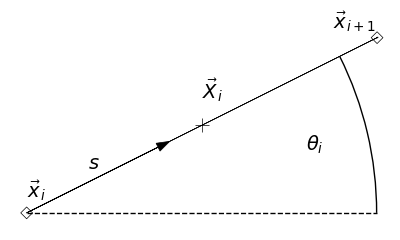
\includegraphics[scale=0.5]{figures/panel.png} \end{center}
\caption{Zur Definition eines Panels}
\label{fig:panel}
\end{figure}
Das Hess-Smith-Panelverfahren ist ein Verfahren zur Berechnung von ebenen Potentialströmungen um geschlossene Körper mit Auftrieb. Ein kontinuierlicher zweidimensionaler Körper mit der Umfangkurve $\mathcal{C}$ wird dabei zunächst durch  $n + 1$ diskrete Datenpunkte $\vec x_i = (x_i, y_i)$ dargestellt. Die Kontur des Profils wird nun durch eine endliche Anzahl Verbindungsgeraden zwischen zwei benachbarten Punkten $\vec x_i, \vec x_{i+1}$, den Panelen $\mathcal{C}_i$ (Abb. \ref{fig:panel}) angenähert. Die Zählrichtung der Punkte sei als gegen den Uhrzeigersinn festgelegt (siehe Abb. \ref{fig:zaehlrichtung}). Für das Profil gilt somit die Periodizität $\vec x_n = \vec x_0$. \\
Jedes Panel wird durch die folgenden Parameter charakterisiert:
\begin{itemize}
\item den Mittelpunkten auf beiden Achsen
\begin{equation}
\label{eq:X}
X_i =  \frac{x_{n-i}+x_{n-i-1}}{2}, \; Y_i =  \frac{y_{n-i}+y_{n-i-1}}{2},
\end{equation}
\item seinem Neigungswinkel
\begin{equation}
\theta_i =  \left( \frac{y_{n-i-1} - y_{n-i}}{x_{n-i-1} - x_{n-i}} \right),
\end{equation}
\item und seiner Länge
\begin{equation}
\label{eq:l}
l_i =  \sqrt{(x_{n-i-1} - x_{n-i})^2 + (y_{n-i-1} - y_{n-i})^2}.
\end{equation}
\end{itemize}



\begin{figure}
\begin{center} 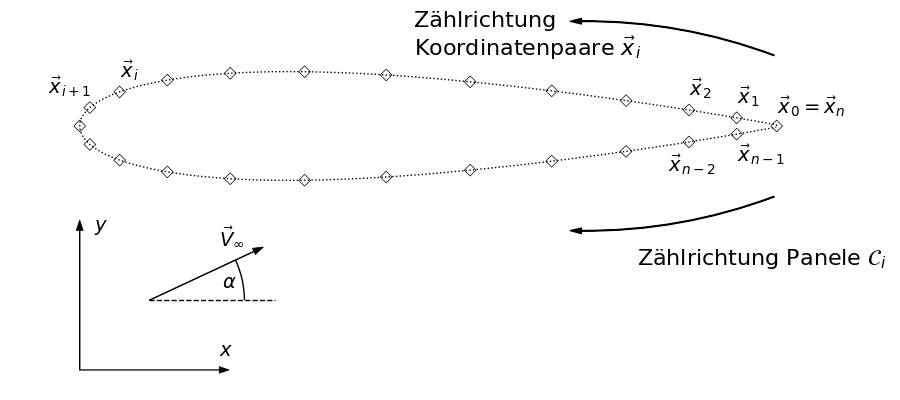
\includegraphics[scale=0.7]{figures/zaehlrichtung.png} \end{center}
\caption{Zur Definition der Zählrichtung für Koordinatenpaare $\vec x = (x,y)$ und Panele $\mathcal{C}_{i}$ sowie der Anströmgeschwindigkeit $V_{\infty}$ und Anströmungswinkel $\alpha$}
\label{fig:zaehlrichtung}
\end{figure}

Die Indexierung der Panele verläuft somit im Uhrzeigersinn. \\
Im Hess-Smith-Panelverfahren sei nun jedes dieser Panele mit einer vorerst unbestimmten, konstanten Quelldichte $q_i$ behaftet, welche an einem Punkt $\vec r_i =  \vec x - \hat x_i(s)$ zum Geschwindigkeitspotential den Beitrag
\begin{equation}
\label{eqn:potq}
\phi_i^{(q)} =  \frac{q_i}{2 \pi } \int_{\mathcal{C_i}} ds \ln r_i
\end{equation}
liefert, mit $s$, der Koordinate der Bogenlänge, welche das Profil parametrisiert. \\
Ebenso liefert die Profilanströmung mit der konstanten Geschwindigkeit $V_{\infty}$ unter dem Winkel $\alpha $ ein Potential
\begin{equation}
\label{eqn:potv}
\phi_{\infty} =  V_{\infty} (\cos{\alpha} x + \sin{\alpha} y).
\end{equation}
Aus der Summe über alle Panelbeiträge aus \eqref{eqn:potq} und \eqref{eqn:potv} ergibt sich das Gesamtgeschwindigkeitspotential zu
\begin{equation}
\label{eqn:potnovortex}
\phi(\vec x) =  V_{\infty} (\cos{\alpha} x + \sin{\alpha} y) + \sum_{i=0}^{n-1} \phi_i^{(q)}.
\end{equation}
Die Geschwindigkeit im Punkt $\vec x$  kann über den Gradienten von $\phi$ berechnet werden:
\begin{equation}
\vec v ( \vec x) =  \nabla  \phi (\vec x).
\end{equation}
Auf der Oberfläche des Profils muss die Strömung die Gleitbedingung erfüllen; damit lassen sich $n$ Gleichungen aufstellen, um diese Bedingung zu modellieren. Es wird gefordert, dass die Normalkomponente des Geschwindigkeitsvektors,
\begin{equation}
v_j^{(n)} =  \vec v(\vec X_j) \cdot \vec n_j,
\end{equation}
verschwindet. Dabei ist $\vec n_j$ der Normalvektor auf das Panel $\mathcal{C}_j$.\\
In 0. Ordnung erhält man ein System von $n$ Gleichungen
\begin{equation}
\label{eq:lgls1}
\sum_{j=0}^{n-1} M_{i,j}^{(q)}q_j =  b_i,
\end{equation}
mit
\begin{equation}
M_{i,j}^{(q)} = \frac{1}{q_j} \nabla \phi_j^{(q)} (\vec X) \cdot \vec n_i,
\end{equation}
und den Inhomogenitäten
\begin{equation}
b_i =  -V_{\infty} \left( \begin{matrix} \cos \alpha \\ \sin \alpha \end{matrix} \right) \cdot \vec n_i,
\end{equation}
aus dessen Lösung die Quellstärken $q_i$ für jedes Panel ermittelt werden können. \\
Damit können die Tangentialkomponenten des Geschwindigkeitsvektors
\begin{equation}
\label{eqn:vt}
v_i^{(t)} =  \vec v(X_i) \cdot \frac{\vec x_{i+1}-\vec x_i}{|\vec x_{i+1}-\vec x_i|},
\end{equation}
bestimmt werden. \\
Aus der Bernoulli-Gleichung
\begin{equation}
p_{\infty} + \frac{1}{2} \rho V_{\infty}^2 =  p + \frac{1}{2} \rho v^2,
\end{equation}
definiert man den Druckbeiwert als das Verhältnis der Druckdifferenzen von Profilanströmung und dynamischem Druck 
\begin{equation}
c_p =  \frac{p-p_{\infty}}{\frac{1}{2} \rho V_{\infty}^2}.
\end{equation}
Daraus kann der Druckbeiwert
\begin{equation}
c_{p_i} =  1 - \left( \frac{v_i^{(t)}}{V_{\infty}}\right)
\end{equation}
am Mittelpunkt des Panels $\mathcal{C}_i$ bestimmt werden. \cite{Hess:1966} \cite{Cebeci:1999} 
\subsection{Berücksichtigung einer Wirbelbelegung}
Will man den Auftrieb berücksichtigen, so reicht die reine Quellbelegung des Profils noch nicht aus. \\
Im Hess-Smith-Verfahren wird für das gesamte Profil eine einzige konstante Wirbelbelegung $\gamma$ für alle Panele angenommen. Damit wird das Potential aus \eqref{eqn:potnovortex} um folgende Beiträge erweitert:
\begin{equation}
\phi_i^{(w)} =  \frac{\gamma}{2 \pi } \int ds \theta_i,
\end{equation}
zu
\begin{align}
\phi(\vec x) &=  V_{\infty} (\cos{\alpha} x + \sin{\alpha} y) + \sum_{i=0}^{n-1} \left( \phi_i^{(q)} + \phi_i^{(w)} \right) \nonumber \\
&= V_{\infty} (\cos{\alpha} x + \sin{\alpha} y) + \sum_{i=0}^{n-1} \int_{\mathcal{C}_i} \left( \frac{q_i}{2\pi } \ln r_i - \frac{\gamma}{2\pi } \theta_{i} \right) ds.
\end{align}
Die Gleitbedingung bleibt erhalten, allerdings muss das Gleichungssystem entsprechend um den hinzugekommenen Geschwindigkeitsbeitrag erweitert werden. Dadurch erhält das Gleichungssystem eine neue Variable $\gamma$ und ist somit unterbestimmt. Die fehlende Gleichung ergibt sich aus der Kutta-Bedingung, welche besagt, dass es an der Hinterkante des Profils keine Umströmung gibt.\\
Zur Modellierung der Kutta-Bedingung wählt man
\begin{equation}
v_0^{(t)} =  -v_n^{(t)}.
\end{equation} 
Daraus folgt, dass die Tangentialkomponenten des Geschwindigkeitsvektors in den Mittelpunkten der Panele, welche die Profilhinterkante bilden, vom Betrag gleich groß und gegenläufig gerichtet sein müssen. %(siehe Abb. \ref{fig:kutta}). 
\\
Nach Lösung des erhaltenen linearen Gleichungssystems mit $q_n = \gamma$ kann nun der Auftriebsbeiwert $c_a$ ermittelt werden. Dieser ergibt sich mit der Proftiltiefe $t$ und der Länge $l_i$ des Panels $\mathcal{C}_i$, approximiert in folgender Form:
\begin{equation}
c_a \approx \frac{2}{V_{\infty}t}\sum_{i=0}^{n-1} v_i^{(t)} l_i.
\end{equation}
%\begin{figure}
%\begin{center} \includegraphics[scale=0.7]{figures/%kutta.png} \end{center}
%\caption{Zur Kutta-Bedingung am Beispiel eines NACA0012-%Profils - am Punkt der Hinterkante sind die %Tangentialgeschwindigkeiten genau entgegengerichtet}
%\label{fig:kutta}
%\end{figure}
Für eine analytische Berechnung des Auftriebsbeiwerts muss nun noch die Systemmatrix bestimmt werden, welche das lineare Gleichungssystem \eqref{eq:lgls1} definiert. \cite{Hess:1966} \cite{Cebeci:1999} \cite{Alonso:2005}

\subsection{Berechnung der Systemmatrix}
\label{chap:systemmatrixtheory}
Die Systemmatrix zur Berechnung der Normalgeschwindigkeiten $v_i^{(n)}$ in den Panelmittelpunkten für eine stückweise konstante Quellenbelegung der Panel ergibt sich aus der Gleitbedingung. Wendet man diese direkt auf \eqref{eqn:potnovortex} an, muss ein kompliziertes Integral gelöst werden. Dieses kann theoretisch mit Computermethoden gelöst werden, für den Berechnungsaufwand ist es allerdings bei Profilen mit einer hohen Anzahl an Panelen günstiger, dieses analytisch zu berechnen. \\
Für die Systemmatrix und ihre Parameter gelten:
\begin{equation}
\label{eq:mnovortex}
M_{i,j} = A_{i,j}^{(n)}, \;\; i = 0, 1, \ldots , n-1; \;\; j = 0,1,\ldots , n-1,
\end{equation}
mit der Einflussmatrix
\begin{equation}
\label{eq:An}
A_{i,j}^{(n)} = -\sin {(\theta _i - \theta _j)} I_{i,j} + \cos{(\theta _i - \theta _j)} J_{i,j},
\end{equation}
sowie den geometrischen Integralen
\begin{equation}
I_{i,j} = 
     \begin{cases}
       \frac{1}{4\pi } \ln \left[ \frac{(l_j + 2 \xi_{i,j})^2 + 4 \eta_{i,j}^2}{(l_j -2 \xi _{i,j})^2 + 4 \eta_{i,j}^2} \right] &\quad i \neq j \\
       0 &\quad i = j \\
     \end{cases},
\end{equation}
und
\begin{equation}
J_{i,j} = 
     \begin{cases}
       \frac{1}{2\pi } \arctan \left[ \frac{l_j - 2 \xi_{i,j}}{2 \eta_{i,j}} \right] + \frac{1}{2\pi } \arctan \left[ \frac{l_j + 2 \xi_{i,j}}{2 \eta_{i,j}} \right] &\quad i \neq j \\
       \frac{1}{2} &\quad i = j \\
     \end{cases}.
\end{equation}
Dabei gilt
\begin{equation}
\label{eq:xi}
\xi_{i,j} =  (X_i - X_j) \cos \theta _j + (Y_i - Y_j) \sin \theta _j;
\end{equation}
\begin{equation}
\label{eq:eta}
\eta_{i,j} =  -(X_i - X_j) \sin \theta _j + (Y_i - Y_j) \cos \theta _j.
\end{equation}
Mit der Systemmatrix und den Inhomogenitäten $b_i$ wird nun das lineare Gleichungssystem aus (\ref{eq:lgls1}) berechnet. \\
Für die Tangentialkomponente der Geschwindigkeit ergibt sich der Ausdruck
\begin{equation}
\label{eq:vtnovortex}
v_i^{(t)} =  \sum_{j=0}^{n-1} A_{i,j}^{(t)} q_j + V_{\infty} \cos{(\alpha - \theta_i)},
\end{equation}
mit der Einflussmatrix
\begin{equation}
\label{eq:At}
A_{i,j}^{(t)} =  \cos{(\theta _i - \theta _j)} I_{i,j} + \sin{(\theta _i - \theta _j)} J_{i,j}.
\end{equation}
\\
Die Systemmatrix $M_{i,j}$ aus \eqref{eq:mnovortex} berücksichtigt allerdings noch keine Wirbelbelegungen und damit keinen Auftrieb.\\
Im Falle einer konstanten Wirbelbelegung $\gamma$ auf allen Panelen erweitert sich die Dimension von $M_{i,j}$ von $n \times n$ auf $(n+1) \times (n+1)$. Dadurch müssen folgende zusätzliche Elemente bestimmt werden:
\begin{equation}
M_{i,n} =  \sum_{j=0}^{n-1} A_{i,j}^{(t)}, \;\; i=0,1,\ldots, n-1;
\end{equation}
\begin{equation}
M_{n,j} =  A_{0,j}^{(t)} + A_{n-1,j}^{(t)}, \;\; j =0,1,\ldots, n-1;
\end{equation}
\begin{equation}
M_{n,n} =  - \sum_{j=0}^{n-1} \left[ A_{0,j}^{(n)} + A_{n-1,j}^{(n)}\right],
\end{equation}
und
\begin{equation}
b_n =  -V_{\infty} [\cos{(\alpha -\theta_0)} + \cos{(\alpha -\theta _{n-1})}].
\end{equation}
Gleichung \eqref{eq:vtnovortex} erweitert sich damit zu
\begin{equation}
\label{eq:vtvortex}
v_i^{(t)} =  \sum_{j=0}^{n-1} A_{i,j}^{(t)} q_j - \gamma \sum_{j=0}^{n-1}A_{i,j}^{(n)} + V_{\infty} \cos{(\alpha - \theta_i)}.
\end{equation}
\cite{Hess:1966} \cite{Cebeci:1999}
\newpage
\chapter{Bericht der Arbeit}
Im Folgenden werden die wesentlichen Erkenntnisse der Arbeit präsentiert.
\section{Vorbereitung der Daten}
Die Daten der Profile wurden der UIUC Airfoil Data Site\footnote{\url{https://m-selig.ae.illinois.edu/ads/coord_database.html}} entnommen und lagen dabei überwiegend im Selig- oder Lednicer-Format vor.\footnote{Eine Gegenüberstellung der beiden Formate ist in \nameref{appendix:a} zu finden.}
\\
Im Lednicer-Format wird in der ersten Zeile die Bezeichnung des Profils angegeben. In der zweiten Zeile wird die Anzahl der Koordinatenpaare der Ober- und Unterseite angegeben. Ab der dritten Zeile werden die Koordinaten der Panelenden $(x_i,y_i)$ von $x=0$ bis $x=1$ für die Oberseite des Profils angegeben. Danach folgt eine Leerzeile. Danach werden die Koordinaten der Panelenden $(x_i,y_i)$ von $x=0$ bis $x=1$ für die Unterseite des Profils angegeben.
\\
Im Selig-Format wird in der ersten Zeile die Bezeichnung des Profils angegeben. Ab der zweiten Zeile werden die Koordinaten der Panelenden $(x_i,y_i)$ im Gegenuhrzeigersinn, beginnend bei $x=1$ angegeben.
\\\\
Es wurde eine Routine implementiert, welche Daten im Lednicer-Format in das Selig-Format überführt. Dies wurde bewerkstelligt, indem die Koordinatenpaare der Oberseite invertiert wurden. Anschließend wurden aus den Daten die Header-Zeilen entfernt. \\
Unter Verwendung der Methode .write\_panels() wurde für die Profile eine .csv-Datei mit den Werten $X_i, Y_i, \theta _i, l_i$ pro Panel erstellt (eine Beispieldatei ist in \nameref{appendix:b} gezeigt). Ebenso wurden Graphen erzeugt, welche sowohl die Geometrie des Profils als auch die Neigungswinkel und Längen der einzelnen Panele darstellen. Zur einfacheren Betrachtung sind die Graphen der Neigungswinkel und Panellängen in die beiden Seiten des Profils aufgeteilt. 
\\Ein solcher Graph ist in Abbildung \ref{fig:naca0012} an einem NACA-0012-Profil gezeigt. Die Symmetrie des Profils spiegelt sich in der gewählten Darstellung der Neigungswinkel und Panellängen wieder.

\begin{figure}
\begin{center}
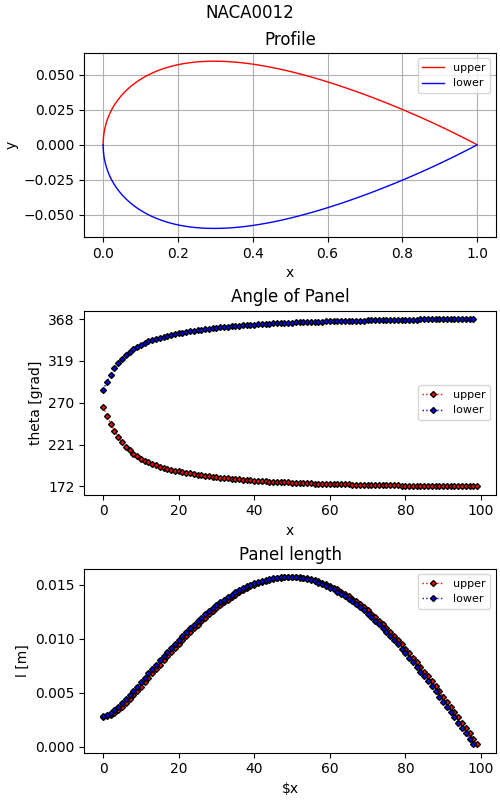
\includegraphics[scale=0.6]{figures/NACA0012.png} 
\caption{NACA-0012-Profil. Aufgrund der Symmetrie des Profils sind die Panellängen für Ober- und Unterseite deckungsgleich}
\label{fig:naca0012}
\end{center}
\end{figure}

\begin{table}
\label{tab:1}
\centering{
\begin{tabular}{cccc}
%\toprule
$X_i$ & $Y_i$         & $\theta_i$ & $l_i$ \\
%\midrule
0.93 & -0.18 & -112.5 & 0.38\\
0.68 & -0.43 & -157.5 & 0.38\\
0.32 & -0.43 & 157.5 & 0.38\\
0.07 & -0.18 & 112.5 & 0.38\\
0.07 & 0.18 & 67.5 & 0.38\\
0.32 & 0.43 & 22.5 & 0.38\\
0.68 & 0.43 & -22.5 & 0.38\\
0.93 & 0.18 & -67.5 & 0.38


%\bottomrule
\end{tabular}
}
\end{table}

\begin{figure}[!h]
\begin{center}
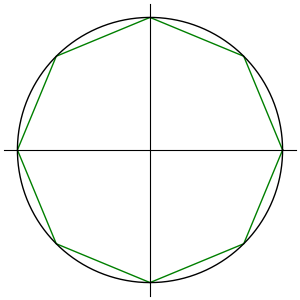
\includegraphics[scale=0.7]{figures/cylinderascircle.png} 
\caption{Achtseitiger Zylinder als Approximation eines Kreiszylinders sowie zugehörige Panelparameter}
\label{fig:cylinder8}
\end{center}
\end{figure}
\section{Untersuchungen am  Kreiszylinder}

Als nächstes wurden Untersuchungen an Kreiszylindern vorgenommen. Zur Generierung der Koordinatenpaare eines Kreiszylinders mit $n$ gleich langen Seiten wurde die Funktion make\_cylinder verwendet (siehe \nameref{appendix:c}). \\
Die Panelparameter sowie die Systemmatrix und sämtliche damit verbundene Werte wurden entsprechend den Gleichungen \eqref{eq:X} bis \eqref{eq:l} sowie \eqref{eq:mnovortex} bis \eqref{eq:vtvortex} berechnet. 

\subsection{Achtseitiger Kreiszylinder}
\subsubsection{Berechnung der Systemmatrix}
Für den in Abbildung \ref{fig:cylinder8} gezeigten Kreisylinder wurde die Systemmatrix (hier gerundet auf zwei Dezimalstellen) zu folgenden Werten berechnet:
\begin{align*}
M_{i,j} = 
\begin{pmatrix}
0.5&0.056&0.064&0.065&0.065&0.065&0.064&0.056 \\
0.056&0.5&0.056&0.064&0.065&0.065&0.065&0.064\\
0.064&0.056&0.5&0.056&0.064&0.065&0.065&0.065\\
0.065&0.064&0.056&0.5&0.056&0.064&0.065&0.065\\
0.065&0.065&0.064&0.056&0.5&0.056&0.064&0.065\\
0.065&0.065&0.065&0.064&0.056&0.5&0.056&0.064\\
0.064&0.065&0.065&0.065&0.064&0.056&0.5&0.056\\
0.056&0.064&0.065&0.065&0.065&0.064&0.056&0.5
\end{pmatrix}
\end{align*}
%\subsubsection{Lösung des wirbelfreien Gleichungssystems}
Im Folgenden wurde die Lösung des linearen Gleichungssystems mit der obigen Systemmatrix und den Inhomogenitäten
\begin{equation}
b_i =  -V_{\infty} \sin{(\alpha -\theta _i)}, \;\; i= 0,1,\ldots, n-1,
\end{equation}
berechnet. Daraus wurde der Vektor der Quellenbelegung zunächst für eine allgemeine Anströmung berechnet: \\
\begin{figure}[!h]
\begin{center}
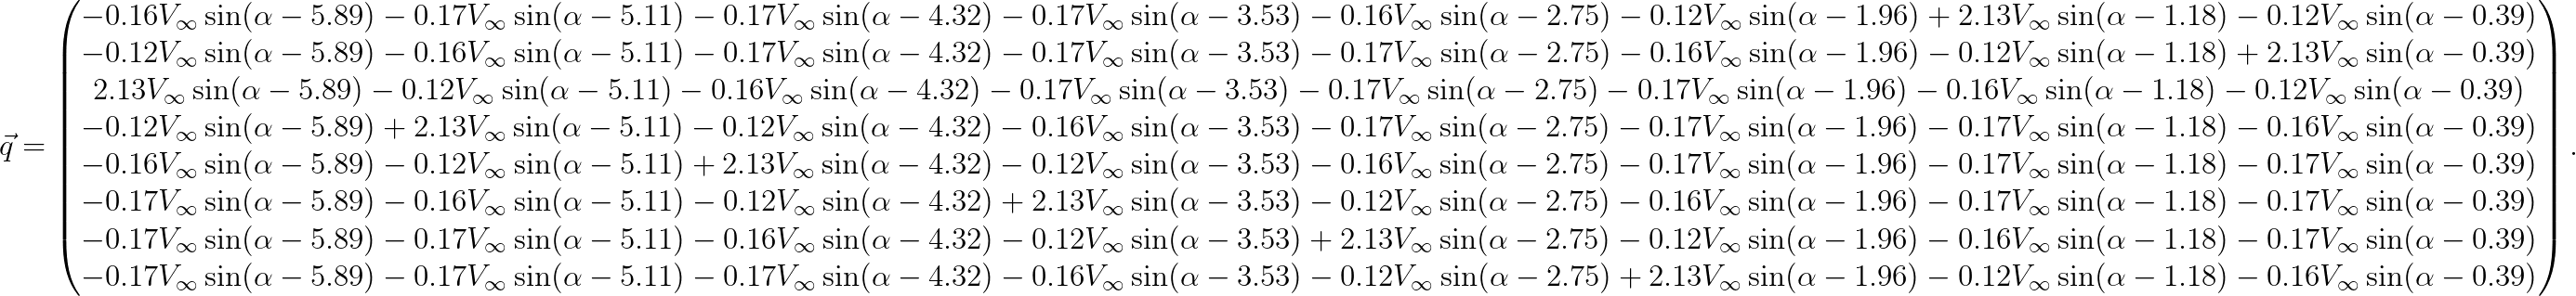
\includegraphics[scale=0.2]{figures/analytical.png} 
\label{fig:analyticalcylinder8}
\end{center}
\end{figure}

Die Ergebnisse für Quellenbelegung, Tangentialgeschwindigkeiten und Druckbeiwerte sind in Tabelle \ref{tab:cyl8} für die Werte $V_{\infty} = 1$ und $\alpha  = 0$ zusammengefasst. \\
Ebenfalls von Interesse ist die Größe $\sum_{i=0}^{n-1} q_i l_i$. Diese Summe sollte für einen geschlossenen Körper Null ergeben, da der Körper sonst durch den Fluss seine Masse verändern würde (vgl. \cite{Barba:2019}). Tatsächlich ergibt sich:
\begin{align*}
\sum_{i=0}^{n-1} q_i l_i \approx 4.44 \cdot 10^{-16}.
\end{align*}
Dieser sehr kleine Fehler beträgt ungefähr zwei Epsilon \footnote{1 Epsilon $=2.220446049250313 \cdot 10^{-16}$ beschreibt die kleinstmögliche in Python darstellbare Gleitkommazahl.  \cite{python2009}} und ergibt sich aus Rundungsfehlern, die bei der Berechnung der Eckpunkte des Kreiszylinders entstehen.

\begin{table}
\caption{Ergebnisse für den achtseitigen Zylinder mit $V_{\infty} = 1, \alpha  = 0$}
\label{tab:cyl8}
\begin{center}
\begin{tabular}{c|ccc}
%\toprule
$i$ & $q_i$ & $v_i^{(t)}$ & $c_{p_i}$ \\
%\midrule
0 & -2.19 & -0.77 & 0.41 \\
1 & -0.91 & -1.85 & -2.41 \\
2 & 0.91 & -1.85 & -2.41 \\
3 & 2.19 & -0.77 & 0.41 \\
4 & 2.19 & 0.77 &  0.41 \\ 
5 &  0.91 & 1.85 & -2.41 \\
6 & -0.91 & 1.85 & -2.41 \\
7 & -2.19 &0.77 & 0.41
%\bottomrule
\end{tabular}
\end{center}
\end{table}

\subsection{Untersuchungen an allgemeinen Kreiszylindern} \label{chap:analyticalcylinder}
Die Potentialtheorie liefert ein exaktes Resultat für den Druckbeiwert auf der Oberfläche eines Zylinders: \cite{Cebeci:1999}
\begin{align}
c_p^\mathrm{exakt} (\varphi ) &=  2 \cos{(2\varphi )} -1.
\end{align}
Dabei bezeichnet $\varphi$ den Winkel der Flächennormale des Kreiszylinders welche ins Innere des Profils zeigt. Mit unserer Definition des Neigungswinkels $\theta$ gilt
\begin{equation}
\varphi = \theta +  \frac{\pi }{2}.
\end{equation}
Abbildung \ref{fig:theoreticalcylinder} zeigt die Abweichung der Druckbeiwerte eines achtseitigen Zylinders vom theoretischen Resultat. Es ergibt sich eine Abweichung dadurch, dass die Mittelpunkte des achtseitigen Zylinders nicht auf der Kreisfläche liegen. Der Fehler ergibt sich zu:
\begin{align}
c_p^\mathrm{exakt} (\varphi ) &=  2 \cos{(2\varphi )} -1 \\
&= 1 - 4 \sin^2 \varphi \\
&= 1 - 4 \left( \frac{Y}{R}\right)^2.
\end{align}
Der Fehler, der bei der Approximation entsteht, ergibt sich folglich zu
\begin{align}
\Delta c_{p_{i}} &= |c_{p_{i}} - c_p^\mathrm{exakt} (\varphi )| \\
&= |c_{p_{i}} -[ 1 - 4 (Y_{i}/R)^2 ] \;|.
\end{align}

\begin{figure}[ht]
  \centering
  \begin{subfigure}[b]{0.5\linewidth}
    \centering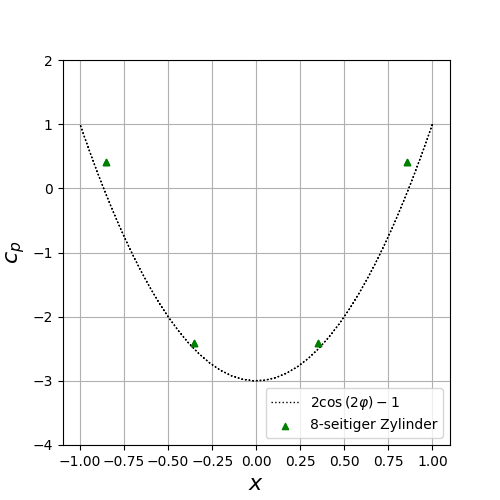
\includegraphics[scale=0.6]{figures/theoretical.png} 
    \caption{\label{fig:theoreticalcylinder}}
  \end{subfigure}%
  \begin{subfigure}[b]{0.5\linewidth}
    \centering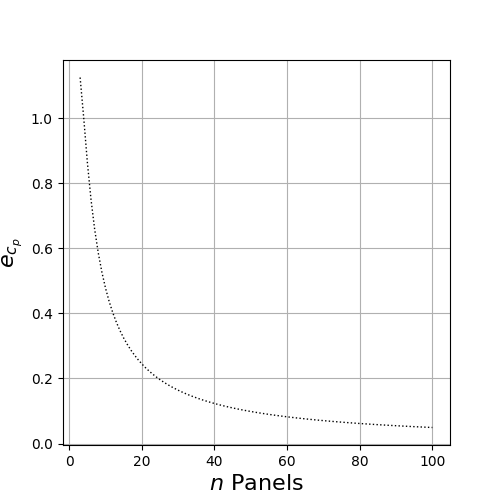
\includegraphics[scale=0.6]{figures/absoluteerror.png} 
    \caption{\label{fig:absoluteerror}}
  \end{subfigure}
  \caption{\subref{fig:theoreticalcylinder}) Abweichung der Druckbeiwerte eines achtseitigen Zylinders vom theoretisch ermittelten Wert \subref{fig:absoluteerror}) Graph der Abweichung des mittleren Fehlers vom exaken Wert.}
\end{figure}
\subsubsection{Variation der Panelanzahl}
Das Programm wurde nun für Kreiszylinder zwischen 5 und 100 Panelen durchlaufen und die mittlere absolute Abweichung $e_{c_p}$ für jeden Kreiszylinder festgehalten (Abbildung \ref{fig:absoluteerror}). Aus den experimentellen Daten wurde mittels Kurvenanpassung für den absoluten Fehler in Abhängigkeit der Panelanzahl $n$ die Beziehung 
\begin{align*}
e_{c_{p}}(n) \approx \frac{17.85301}{n^2} + 0.00183,
\end{align*}
ermittelt.

\subsubsection{Rotation des achtseitigen Zylinders}
Als nächstes wurden die Werte $\gamma$, $c_a$, sowie die Druckbeiwerte für verschiedene Winkel im Bereich $\alpha \in [-15^{\circ}, 15^{\circ}]$ bestimmt. Die Ergebnisse sind in Tabelle \ref{tab:cylgammacas} aufgetragen. 

\begin{table}
\caption{Ergebnisse für den achtseitigen Zylinder mit $V_{\infty} = 1, \alpha  \in [-15^{\circ}, 15^{\circ}]$}
\label{tab:cylgammacas}
\centering{
\begin{tabular}{c|cc|cccccccc}
%\toprule
$\alpha$ & $\gamma$ & $c_a$ & $c_{p_0}$ & $c_{p_1}$& $c_{p_{2}}$& $c_{p_3}$& $c_{p_4}$& $c_{p_5}$& $c_{p_6}$& $c_{p_7}$ \\
%\midrule
-15 & 0.51 & -2.93 & 0.45 & -3.26 & -5.06 & -1.88 & 0.95 & -0.23 & -1.26 & 0.45 \\ 
-14 & 0.48 & -2.74 & 0.45 & -3.22 & -4.88 & -1.68 & 0.98 & -0.35 & -1.34 & 0.45 \\ 
-13 & 0.44 & -2.55 & 0.44 & -3.18 & -4.7 & -1.49 & 0.99 & -0.47 & -1.42 & 0.44 \\ 
-12 & 0.41 & -2.35 & 0.44 & -3.13 & -4.53 & -1.3 & 1.0 & -0.6 & -1.5 & 0.44 \\ 
-11 & 0.38 & -2.16 & 0.44 & -3.08 & -4.35 & -1.12 & 1.0 & -0.73 & -1.58 & 0.44 \\ 
-10 & 0.34 & -1.96 & 0.43 & -3.03 & -4.17 & -0.95 & 0.99 & -0.87 & -1.66 & 0.43 \\ 
-9 & 0.31 & -1.77 & 0.43 & -2.98 & -3.99 & -0.78 & 0.97 & -1.01 & -1.74 & 0.43 \\ 
-8 & 0.28 & -1.57 & 0.43 & -2.92 & -3.81 & -0.62 & 0.94 & -1.15 & -1.82 & 0.43 \\ 
-7 & 0.24 & -1.38 & 0.42 & -2.86 & -3.63 & -0.46 & 0.9 & -1.3 & -1.9 & 0.42 \\ 
-6 & 0.21 & -1.18 & 0.42 & -2.81 & -3.46 & -0.32 & 0.86 & -1.45 & -1.97 & 0.42 \\ 
-5 & 0.17 & -0.99 & 0.42 & -2.74 & -3.28 & -0.18 & 0.81 & -1.6 & -2.05 & 0.42 \\ 
-4 & 0.14 & -0.79 & 0.42 & -2.68 & -3.1 & -0.04 & 0.74 & -1.76 & -2.12 & 0.42 \\ 
-3 & 0.1 & -0.59 & 0.42 & -2.62 & -2.93 & 0.08 & 0.67 & -1.92 & -2.2 & 0.42 \\ 
-2 & 0.07 & -0.39 & 0.41 & -2.55 & -2.76 & 0.2 & 0.6 & -2.08 & -2.27 & 0.41 \\ 
-1 & 0.03 & -0.2 & 0.41 & -2.48 & -2.58 & 0.31 & 0.51 & -2.25 & -2.34 & 0.41 \\ 
0 & -0.0 & 0.0 & 0.41 & -2.41 & -2.41 & 0.41 & 0.41 & -2.41 & -2.41 & 0.41 \\ 
1 & -0.03 & 0.2 & 0.41 & -2.34 & -2.25 & 0.51 & 0.31 & -2.58 & -2.48 & 0.41 \\ 
2 & -0.07 & 0.39 & 0.41 & -2.27 & -2.08 & 0.6 & 0.2 & -2.76 & -2.55 & 0.41 \\ 
3 & -0.1 & 0.59 & 0.42 & -2.2 & -1.92 & 0.67 & 0.08 & -2.93 & -2.62 & 0.42 \\ 
4 & -0.14 & 0.79 & 0.42 & -2.12 & -1.76 & 0.74 & -0.04 & -3.1 & -2.68 & 0.42 \\ 
5 & -0.17 & 0.99 & 0.42 & -2.05 & -1.6 & 0.81 & -0.18 & -3.28 & -2.74 & 0.42 \\ 
6 & -0.21 & 1.18 & 0.42 & -1.97 & -1.45 & 0.86 & -0.32 & -3.46 & -2.81 & 0.42 \\ 
7 & -0.24 & 1.38 & 0.42 & -1.9 & -1.3 & 0.9 & -0.46 & -3.63 & -2.86 & 0.42 \\ 
8 & -0.28 & 1.57 & 0.43 & -1.82 & -1.15 & 0.94 & -0.62 & -3.81 & -2.92 & 0.43 \\ 
9 & -0.31 & 1.77 & 0.43 & -1.74 & -1.01 & 0.97 & -0.78 & -3.99 & -2.98 & 0.43 \\ 
10 & -0.34 & 1.96 & 0.43 & -1.66 & -0.87 & 0.99 & -0.95 & -4.17 & -3.03 & 0.43 \\ 
11 & -0.38 & 2.16 & 0.44 & -1.58 & -0.73 & 1.0 & -1.12 & -4.35 & -3.08 & 0.44 \\ 
12 & -0.41 & 2.35 & 0.44 & -1.5 & -0.6 & 1.0 & -1.3 & -4.53 & -3.13 & 0.44 \\ 
13 & -0.44 & 2.55 & 0.44 & -1.42 & -0.47 & 0.99 & -1.49 & -4.7 & -3.18 & 0.44 \\ 
14 & -0.48 & 2.74 & 0.45 & -1.34 & -0.35 & 0.98 & -1.68 & -4.88 & -3.22 & 0.45 \\ 
15 & -0.51 & 2.93 & 0.45 & -1.26 & -0.23 & 0.95 & -1.88 & -5.06 & -3.26 & 0.45 \\ 


%\bottomrule
\end{tabular}
}
\end{table}

\section{Auswertung ausgewählter Profile}
\label{chap:profilauswertung}
Im Folgenden wurde das entwickelte Programm auf die drei Profile NACA-0012, NASA SC(2)-0614 und Taylor Zone-40 angewandt. Für jedes Profil wurden die Werte $\gamma$ und $c_a$ unter verschiedenen Anströmwinkeln $\alpha $ berechnet. \\
An dieser Stelle wurde das Programm um die Möglichkeit erweitert, den Geschwindigkeitsvektor an jedem Punkt des Profils zu berechnen. Dies spiegelt sich in \eqref{eq:xi} und \eqref{eq:eta} wieder, für welche dann
\begin{equation}
\xi_{j} =  (x - X_j) \cos \theta _j + (y - Y_j) \sin \theta _j,
\end{equation}
und
\begin{equation}
\eta_{j} =  -(x - X_j) \sin \theta _j + (y - Y_j) \cos \theta _j,
\end{equation}
gelten. \eqref{eq:An} und \eqref{eq:At} vereinfachen sich ebenfalls zu
\begin{equation}
A_{j}^{(n)} = \sin {(\theta _j)} I_{j} + \cos{( \theta _j)} J_{j};
\end{equation}
\begin{equation}
A_{j}^{(t)} =  \cos{(\theta _j)} I_{j} - \sin{( \theta _j)} J_{j}.
\end{equation}
Der Geschwindigkeitsvektor im Punkt $\vec x = (x,y)$ ergibt sich also zu:
\begin{equation}
\vec v (x,y) = 
\begin{pmatrix}
v_x \\
v_y
\end{pmatrix}
=
\begin{pmatrix}
\sum_{j=0}^{n-1} A_{j}^{(t)} q_j - \gamma \sum_{j=0}^{n-1}A_{j}^{(n)} + V_{\infty} \cos{(\alpha)} \\
\sum_{j=0}^{n-1} A_{j}^{(n)} q_j + \gamma \sum_{j=0}^{n-1}A_{j}^{(t)} + V_{\infty} \cos{(\alpha)}
\end{pmatrix}.
\end{equation}
Diese Geschwindigkeitsvektoren wurden für die oben genannten Profile für ein Gitter der Dimension $200 \times 200$ und den Punkten
\begin{align*}
\vec x = (x,y) = \{-0.5, -0.5 + n \Delta x,\ldots, 1,5\} \times \{-0.2, -0.2 + n \Delta y, \ldots, 0.2\}; \\ \;\; \Delta x = \frac{1.5 - (-0.5)}{200}, \;\; \Delta y = \frac{0.2 - (-0.2)}{200}, \;\; n \in \mathbb{N} \cap (0,200),
\end{align*} 
berechnet und sind in Form eines Strömungsgraphens dargestellt. Auch wurde ein Konturgraph für die sich ergebenden Druckbeiwerte im Umgebungsfeld des Profils generiert. \\
Ebenfalls wurden in Form eines Farbgraphens für die Panele die Werte für Quellbelegung und Druckbeiwerte auf der Profiloberfläche ermittelt und dargestellt. Für sämtliche oben genannten Graphen wurde für die Anströmgeschwindigkeit $V_{\infty} = 1$, für den Anströmwinkel $\alpha =5^{\circ}$ gewählt.

\newpage
\subsection{NACA-0012-Profil} 
\begin{minipage}{0.45\textwidth}
\begin{table}[H]
    \centering
    \begin{tabular}{c|cc}
    $\alpha$ & $\gamma$ & $c_a$ \\
        -11 & 0.32 & -1.32 \\ 
-7 & 0.21 & -0.84 \\ 
-3 & 0.09 & -0.36 \\ 
1 & -0.03 & 0.12 \\ 
5 & -0.15 & 0.6 \\ 
9 & -0.27 & 1.08 \\ 
13 & -0.38 & 1.55 \\ 
17 & -0.5 & 2.02 \\ 

    \end{tabular}
    \label{tab:naca}
    \caption{Ergebnisse des NACA-0012-Profils}
\end{table}
\end{minipage}
\hfill
\begin{minipage}{0.45\textwidth}
\begin{figure}[H]
    \centering
    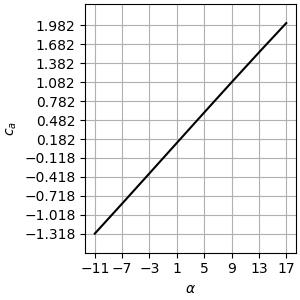
\includegraphics[scale=0.6]{figures/nacaca.png}
    \caption{Graph des Auftriebsbeiwerts}
    \label{fig:nacaca}
\end{figure}
\end{minipage}

\begin{figure*}[!ht]
  \centering
  \begin{subfigure}[b]{0.475\linewidth}
    \centering\includegraphics[scale=0.5]{figures/naca0012stream.png} 
    \caption{\label{fig:nacastream}}
  \end{subfigure}
  \hfill
  \begin{subfigure}[b]{0.475\linewidth}
    \centering\includegraphics[scale=0.5]{figures/naca0012contourcp.png} 
    \caption{\label{fig:nacacontourcp}}
  \end{subfigure}
  \vskip\baselineskip
  \begin{subfigure}[b]{0.475\linewidth}
    \centering\includegraphics[scale=0.5]{figures/naca0012q.png} 
    \caption{\label{fig:nacaq}}
  \end{subfigure}
  \hfill
  \begin{subfigure}[b]{0.475\linewidth}
    \centering\includegraphics[scale=0.5]{figures/naca0012cp.png} 
    \caption{\label{fig:nacacp}}
  \end{subfigure}
  
  \caption{\subref{fig:nacastream}) Umströmung und \subref{fig:nacacontourcp}) Druckbeiwerte im Feld \subref{fig:nacaq}) Quellbelegung und \subref{fig:nacacp}) Druckbeiwerte pro Panel $\mathcal{C}_{i}$ unter dem Anströmwinkel $\alpha =5^{\circ}$}
\end{figure*}

\newpage
\subsection{NASA SC(2)-0614-Profil}
\begin{minipage}{0.45\textwidth}
\begin{table}[H]
    \centering
    \begin{tabular}{c|cc}
    $\alpha$ & $\gamma$ & $c_a$ \\
        -11 & 0.3 & -1.26 \\ 
-7 & 0.19 & -0.77 \\ 
-3 & 0.07 & -0.27 \\ 
1 & -0.05 & 0.22 \\ 
5 & -0.17 & 0.71 \\ 
9 & -0.29 & 1.2 \\ 
13 & -0.41 & 1.69 \\ 
17 & -0.53 & 2.16 \\ 

    \end{tabular}
    \label{tab:nlf}
    \caption{Ergebnisse des NASA SC(2)-0614-Profils}
\end{table}
\end{minipage}
\hfill
\begin{minipage}{0.45\textwidth}
\begin{figure}[H]
    \centering
    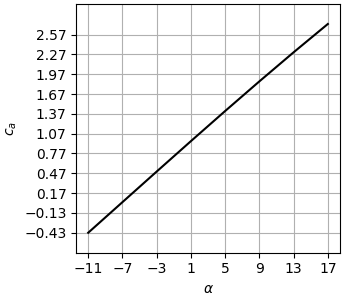
\includegraphics[scale=0.6]{figures/nlf105ca.png}
    \caption{Graph des Auftriebsbeiwerts}
    \label{fig:nlfca}
\end{figure}
\end{minipage}

\begin{figure*}[!ht]
  \centering
  \begin{subfigure}[b]{0.475\linewidth}
    \centering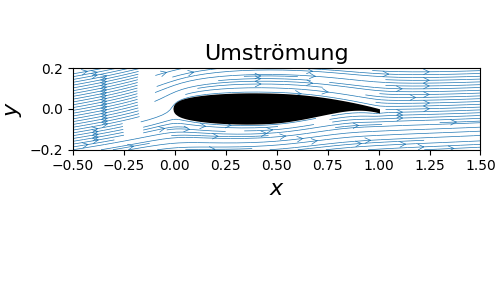
\includegraphics[scale=0.5]{figures/sc20614stream.png} 
    \caption{\label{fig:sc20614stream}}
  \end{subfigure}
  \hfill
  \begin{subfigure}[b]{0.475\linewidth}
    \centering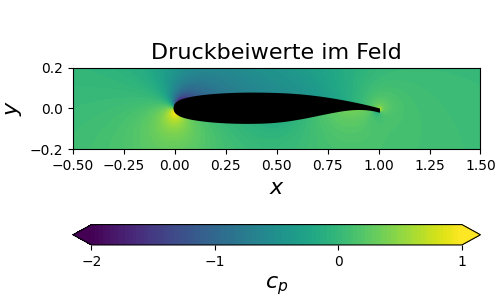
\includegraphics[scale=0.5]{figures/sc20614contourcp.png} 
    \caption{\label{fig:sc20614contourcp}}
  \end{subfigure}
  \vskip\baselineskip
  \begin{subfigure}[b]{0.475\linewidth}
    \centering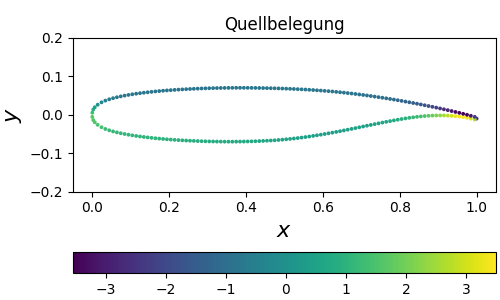
\includegraphics[scale=0.5]{figures/sc20614q.png} 
    \caption{\label{fig:sc20614q}}
  \end{subfigure}
  \hfill
  \begin{subfigure}[b]{0.475\linewidth}
    \centering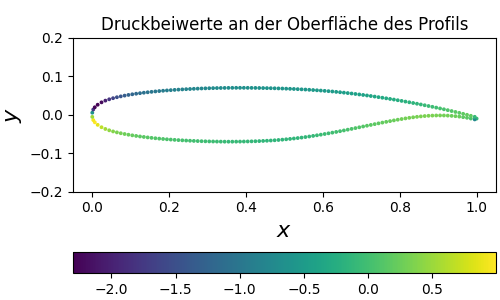
\includegraphics[scale=0.5]{figures/sc20614cp.png} 
    \caption{\label{fig:sc20614cp}}
  \end{subfigure}
  
  \caption{\subref{fig:sc20614stream}) Umströmung und \subref{fig:sc20614contourcp}) Druckbeiwerte im Feld \subref{fig:sc20614q}) Quellbelegung und \subref{fig:sc20614cp}) Druckbeiwerte pro Panel $\mathcal{C}_{i}$ unter dem Anströmwinkel $\alpha =5^{\circ}$}
\end{figure*}
\newpage
\subsection{Taylor Zone-40-Profil}

\begin{minipage}{0.45\textwidth}
\begin{table}[H]
    \centering
    \begin{tabular}{c|cc}
    $\alpha$ & $\gamma$ & $c_a$ \\
        -11 & 0.31 & -1.23 \\ 
-7 & 0.19 & -0.78 \\ 
-3 & 0.08 & -0.32 \\ 
1 & -0.04 & 0.14 \\ 
5 & -0.15 & 0.59 \\ 
9 & -0.27 & 1.05 \\ 
13 & -0.38 & 1.49 \\ 
17 & -0.49 & 1.94 \\ 

    \end{tabular}
    \label{tab:zone}
    \caption{Ergebnisse des Taylor Zone-40-Profils}
\end{table}
\end{minipage}
\hfill
\begin{minipage}{0.45\textwidth}
\begin{figure}[H]
    \centering
    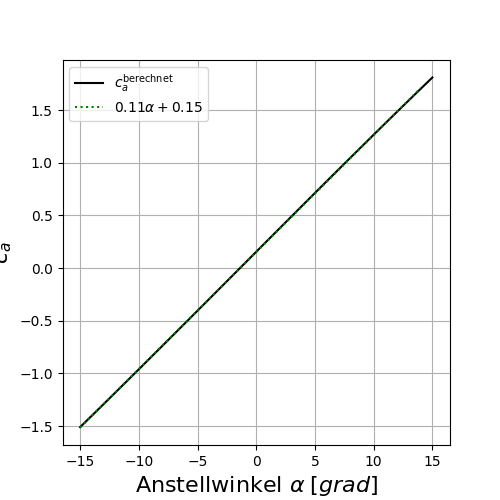
\includegraphics[scale=0.6]{figures/zoneca.png}
    \caption{Graph des Auftriebsbeiwerts}
    \label{fig:zoneca}
\end{figure}
\end{minipage}

\begin{figure*}[!ht]
  \centering
  \begin{subfigure}[b]{0.475\linewidth}
    \centering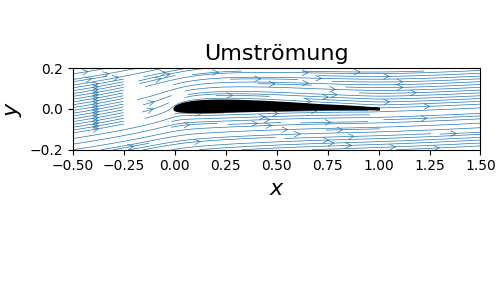
\includegraphics[scale=0.5]{figures/z40stream.png} 
    \caption{\label{fig:zonestream}}
  \end{subfigure}
  \hfill
  \begin{subfigure}[b]{0.475\linewidth}
    \centering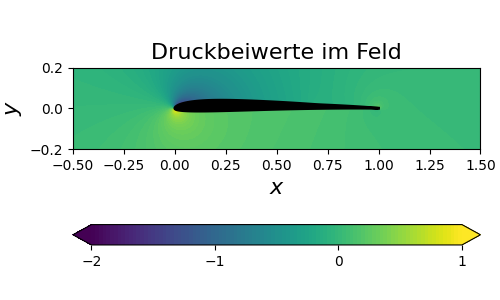
\includegraphics[scale=0.5]{figures/z40contourcp.png} 
    \caption{\label{fig:zonecontourcp}}
  \end{subfigure}
  \vskip\baselineskip
  \begin{subfigure}[b]{0.475\linewidth}
    \centering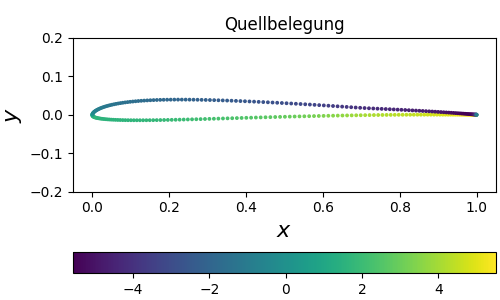
\includegraphics[scale=0.5]{figures/z40q.png} 
    \caption{\label{fig:zoneq}}
  \end{subfigure}
  \hfill
  \begin{subfigure}[b]{0.475\linewidth}
    \centering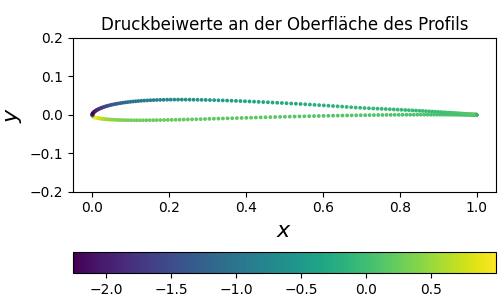
\includegraphics[scale=0.5]{figures/z40cp.png} 
    \caption{\label{fig:zonecp}}
  \end{subfigure}
  
  \caption{\subref{fig:zonestream}) Umströmung und \subref{fig:zonecontourcp}) Druckbeiwerte im Feld \subref{fig:zoneq}) Quellbelegung und \subref{fig:zonecp}) Druckbeiwerte pro Panel $\mathcal{C}_{i}$ unter dem Anströmwinkel $\alpha =5^{\circ}$}
\end{figure*}


\newpage
\section{Abschätzung der Fehlerordnung anhand des Joukowski-Profils}
\begin{figure}[]
  \centering
  \begin{subfigure}[b]{0.5\linewidth}
    \centering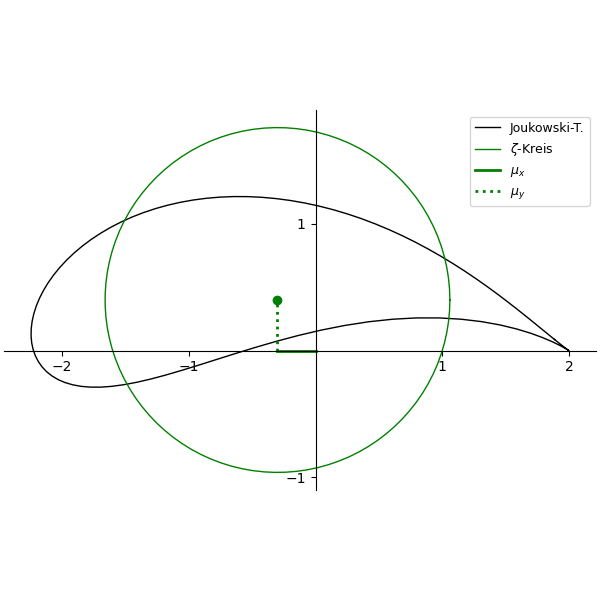
\includegraphics[scale=0.45]{figures/joukowskitrans.png} 
    \caption{\label{fig:joukowskitrans}}
  \end{subfigure}%
  \begin{subfigure}[b]{0.5\linewidth}
    \centering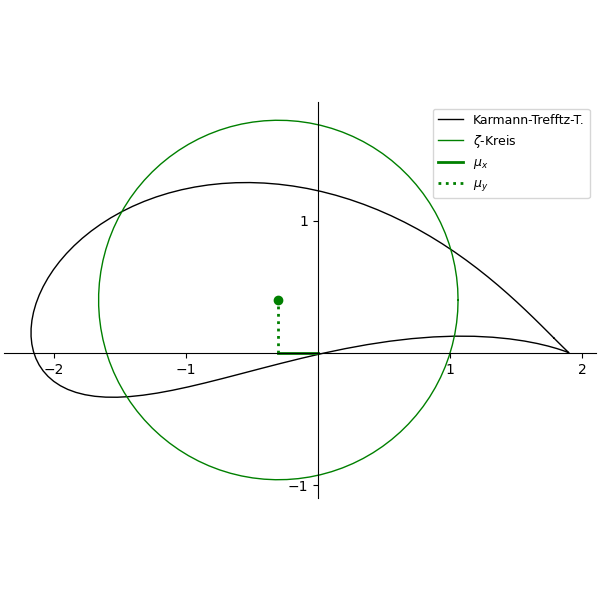
\includegraphics[scale=0.45]{figures/karmantrefftztrans.png} 
    \caption{\label{fig:karmantrefftztrans}}
  \end{subfigure}
  \caption{Vergleich der \subref{fig:joukowskitrans}) Joukowski-Transformation mit der \subref{fig:karmantrefftztrans}) Kármán-Trefftz-Transformation. Für beide Transformationen wurde $\mu_x = 0.3, \mu_y =0.4$ gewählt; für die Kármán-Trefftz-Transformation wurde $n=1.9$ gesetzt.\label{fig:joukar}}
\end{figure}
Die Joukowski-Transformation ist eine konforme Abbildung, deren Transformation als Ergebnis Tragflächenprofile liefert. Die Transformationsgleichung lautet:
\begin{equation}
\label{eq:joukowski}
z = \zeta + \frac{a^2}{\zeta},
\end{equation}
mit einem reellen Parameter $a$ welcher im Folgenden $a=1$ gesetzt wird. Dabei ist $z = x + iy$ eine komplexe Zahl im Bildraum und $\zeta = \chi + i \eta$ eine komplexe Zahl im Ursprungsraum. \\
Ein Joukowski-Profil wird im $z$-Raum durch die Anwendung der Joukowski-Transformation auf einen Kreis im $\zeta$-Raum erzeugt. Einsetzen von $z$ und $\zeta$ in \eqref{eq:joukowski} ergibt die realen und imaginären Komponenten
\begin{equation}
x={\frac {\chi \left(\chi ^{2}+\eta ^{2}+1\right)}{\chi ^{2}+\eta ^{2}}}, \;\;\; y={\frac {\eta \left(\chi ^{2}+\eta ^{2}-1\right)}{\chi ^{2}+\eta ^{2}}}.
\end{equation}
Durch Verschiebung des Mittelpunkts des Kreises in der $\zeta$-Ebene können so verschieden Profile generiert werden. Die Abbildung hat allerdings an den Stellen $z = \pm a = \pm 1$ eine Singularität. Deshalb legt man einen der Punkte (hier $z = -1$) ins Innere des Kreises und den Punkt $z=1$ auf den Kreis. In diesem Fall ergibt sich an der Hinterkante ein Winkel von $0^{\circ}$. \\
\begin{figure}[!ht]
\begin{center} 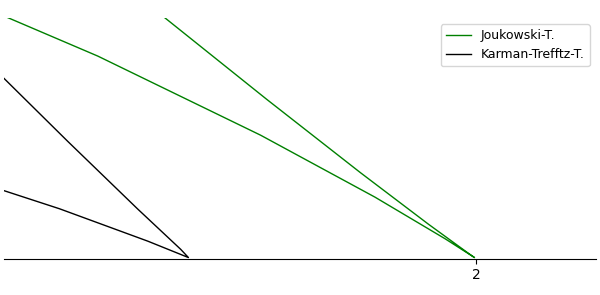
\includegraphics[scale=0.5]{figures/zoomedjouk.png} \end{center}
\caption{Vergleich der Hinterkantenwinkel des Joukowski- und Kármán-Trefftz-Profils}
\label{fig:zoomedjouk}
\end{figure}
\\
Ein Profil mit einem Winkel ungleich Null an der Hinterkante lässt sich durch eine verwandte Transformation, die Kármán-Trefftz-Transformation
\begin{equation}
z=nb{\frac {(\zeta +b)^{n}+(\zeta -b)^{n}}{(\zeta +b)^{n}-(\zeta -b)^{n}}},
\end{equation}
erzeugen, wiederum mit einem reellen Parameter $b$ (im Folgenden $b=1$) und $n \in [1,2]$, wobei sich für $n=1$ der Kreis in der $\zeta$-Ebene und für $n=2$ die Joukowski-Transformation ergibt. Die beiden Transformationen sind in Abbildung \ref{fig:joukar} unter gleichen Parametern dargestellt. Abbildung \ref{fig:zoomedjouk} gibt einen näheren Blick auf die Profilhinterkante. \\
Die analytische Lösung einer ebenen Potentialströmung um einen Kreiszylinder ist bekannt (siehe \ref{chap:analyticalcylinder}). Damit ist auch eine Lösung für Joukowski-Profile gegeben. Für die Zirkulation $\Gamma = \sum_{i=1}^{n-1} \gamma l_i$ ergibt sich
\begin{equation}
\Gamma = 4  V_{\infty}R \sin{\left(\alpha + \arcsin \frac{\mu_y}{R} \right)}.
\end{equation}
Mit dem Kutta-Joukowski-Theorem für den dynamischen Auftrieb $F_a = \rho \Gamma V_{\infty}$ ist über den dynamischen Auftrieb mit $c_a = \tfrac{F_a}{pt} = \tfrac{2F_a}{\rho V_{\infty}}$ ein Ausdruck für den Auftriebsbeiwert gegeben:
\begin{equation}
\label{eq:joukowskitheoretical}
c_a = \frac{8  R V_{\infty} \sin{\left(\alpha + \arcsin \frac{\mu_y}{R} \right)}}{V_{\infty}t}.
\end{equation} 
Es wurde nun für Joukowski-Profile mit den Parametern $\mu_x = 0.2, \mu_y =0.1$ für 10 bis 200 Panele der Auftriebsbeiwert berechnet und mit dem theoretischen Resultat aus \eqref{eq:joukowskitheoretical} verglichen. 
\begin{figure}[!ht]
\begin{center} 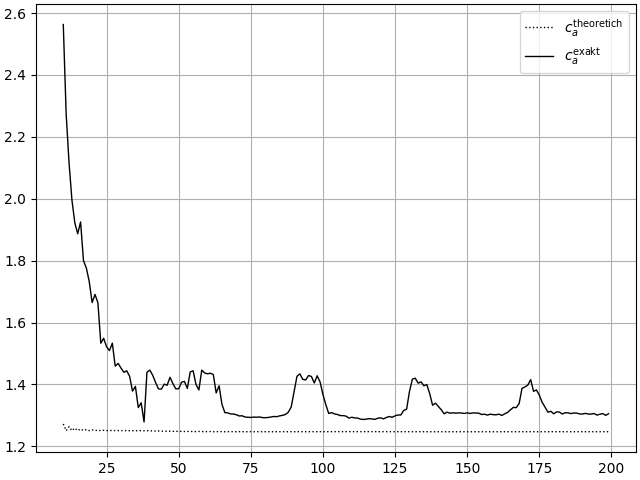
\includegraphics[scale=0.5]{figures/joukowskierror.png} \end{center}
\caption{Vergleich des theoretisch ermittelten Werts für den Auftriebsbeiwert eines Joukowski-Profils mit $\mu_x = 0.2, \mu_y =0.1$ und dem berechneten Wert.}
\label{fig:joukowskitheoretical}
\end{figure}
Es ist ersichtlich, dass sich der Auftriebsbeiwert ab einer Panelanzahl von ungefähr 75 stabil eingeschwungen hat, bis auf Schwankungen, welche vermutlich auf der Diskretisierungsfunktion des Joukowski-Profils beruhen. Für den mittleren relativen Fehler eines Joukowski-Profils mit mindestens 75 Panelen wurde der Wert
\begin{align*}
\frac{\Delta c_a}{c_a^\mathrm{theoretisch}} &= \frac{|c_a^\mathrm{theoretisch} - c_a^\mathrm{exakt}|}{c_a^\mathrm{theoretisch}} \\
& = 0.033 = 3.3 \%,
\end{align*}
ermittelt. \cite{Abello2018} \cite{Barba:2019}
%\begin{figure}[!ht]
%\begin{center} 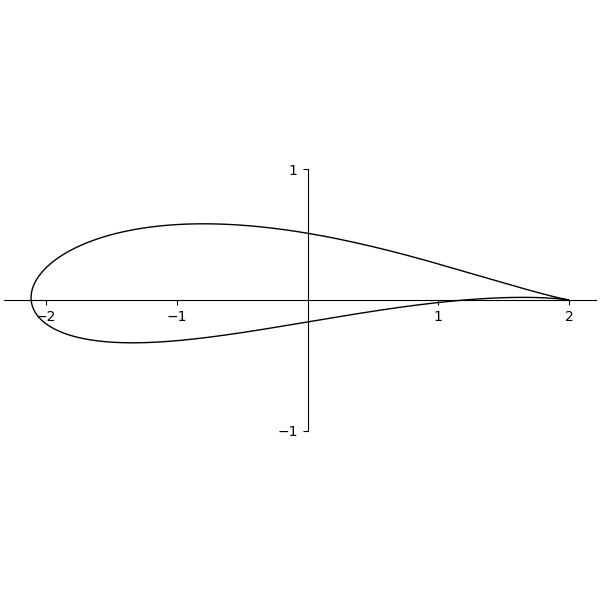
\includegraphics[scale=0.3]{figures/jouk0201.png} \end{center}
%\caption{Joukowski-Profil, $\mu_x = 0.2, \mu_y =0.1$}
%\label{fig:jouk0201}
%\end{figure}